\section{Loss Spikes and Functional Oscillations under Adam}
\label{sec:adam}\label{sec:adam-diagnostics}

The preceding experiments show why consecutive steps must be considered
together. Reversal describes opposition; gradient growth determines its
size. Under SGD the raw gradients also determine the applied increments.
Adam combines the current gradient with past gradients and rescales
coordinates using second moments~\cite{kingma2014adam}. Its recurrences are
\begin{equation}
 \begin{aligned}
 m_t&=\beta_1m_{t-1}+(1-\beta_1)g_t,\\
 v_t&=\beta_2v_{t-1}+(1-\beta_2)g_t^{\odot2}.
 \end{aligned}
 \label{eq:adam-moments}
\end{equation}
The bias-corrected direction and parameter update are
\begin{equation}
 d_t=\frac{m_t/(1-\beta_1^{t+1})}
 {\sqrt{v_t/(1-\beta_2^{t+1})}+\epsilon},\qquad
 \theta_{t+1}=\theta_t-\eta_t d_t.
 \label{eq:adam-update}
\end{equation}
Moments start at zero before $t=0$, and the operations on second moments
are coordinatewise. The experiments use the native Adam update with
$(\beta_1,\beta_2)=(.9,.999)$ and $\epsilon=10^{-8}$, without weight decay.
The Adam overview uses 1,024 full-batch updates per model, with learning rates
of $0.001$ for the MLP and $0.003$ for both ResNet-32 and the Transformer.

Although Adam transforms the raw gradient, consecutive gradients are
evaluated at states separated by the actual Adam update. Their alignment
and relative magnitudes therefore characterize the gradient response
along the trajectory followed by the optimizer (Appendix~\ref{app:math}).

We first characterize the gradient response along Adam's trajectory,
then trace the corresponding functional changes through the network.
The following section tests interventions from matched training states.
The complete experimental grid is specified in Appendix~\ref{app:validation}.

\subsection{Characterizing Loss Spikes}
\label{subsec:characterization}

\begin{figure*}[!t]
\centering
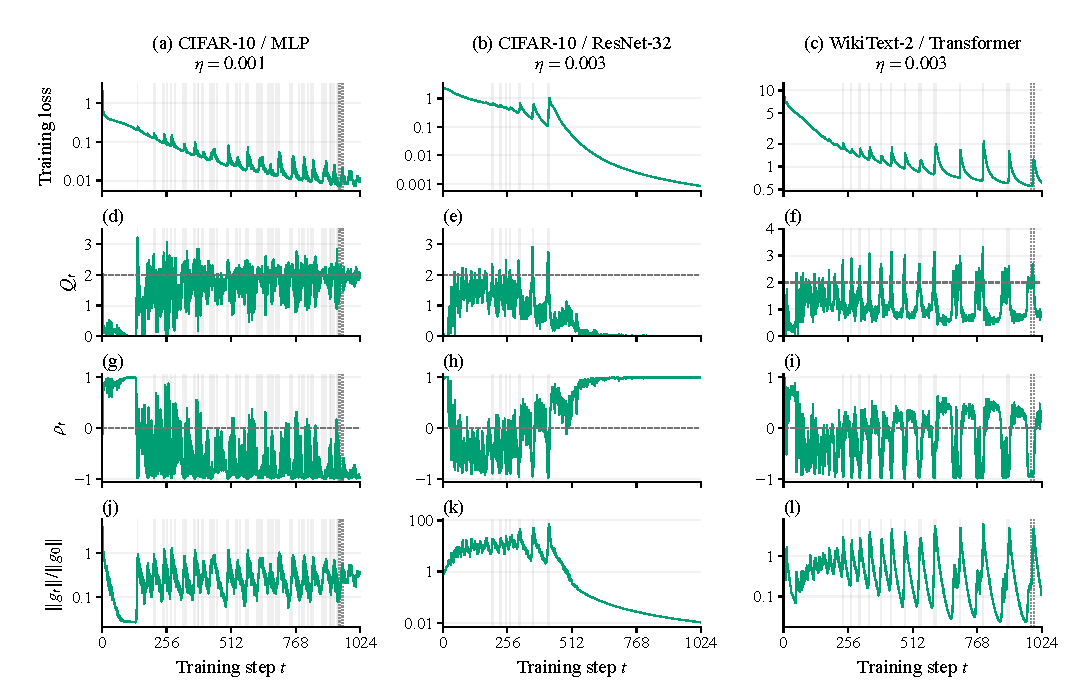
\includegraphics[width=\textwidth]{figures/00-high-lr-overview-cifar10-mlp-resnet-wikitext2-transformer.pdf}
\caption{Loss spikes and consecutive-gradient behavior under full-objective Adam. Columns are MLP, ResNet-32, and Transformer, at learning rates $.001/.003/.003$, with one initialization per model. Rows show loss, the gradient-projected response $\eta\widehat\kappa_t$, consecutive-gradient cosine, and gradient norm relative to initialization. Filled gray bands mark the rising portions of recovered loss excursions exceeding 10\%; outlined bands mark excursions whose recovery is not observed. Events are selected from loss alone. Training step $t$ counts completed updates; gradient measurements are made at $\theta_t$, before the next update. Loss is recorded through 1,024 updates and gradients through 1,023. The $\eta\widehat\kappa_t$ axis starts at zero; negative values lie outside its displayed range.}
\label{fig:adam-overview}
\end{figure*}

Unlike the sustained GD oscillations, the Adam trajectories exhibit
distinct excursions and recoveries. This is consistent with the adaptive
preconditioner mechanism analyzed by Bai et al.~\cite{bai2026spikes}:
changing second moments can alter the effective step size independently
of changes in the underlying Hessian. Our measurements describe how the
resulting motion appears in consecutive gradients. Early constructive
intervals give way to persistent reversal.
Prominent excursions occur with negative cosine and growing gradient
norms, producing large peaks in $\eta\widehat\kappa_t$. In ResNet and
Transformer, recovery often includes renewed constructive alignment and
falling norms.

The loss can reach lower values after an excursion. Such an excursion
could accompany movement into another basin, while momentum can delay
the update's response to a newly changing gradient direction. Whether
that movement helps depends on the current landscape, architecture,
and optimizer state. Related work on SGD catapults shows that spikes can
accompany improved feature learning~\cite{zhu2024catapults}; their role
under Adam must likewise be evaluated together with subsequent progress.

After computing the raw gradient, but before applying the next update,
we may want to classify whether that update will increase the loss.
Let $L_t=\mathcal L(\theta_t)$ and define an increase as
$(L_{t+1}-L_t)/L_t\geq0.001$. At decision step $t$, both $g_t$ and $L_t$
are available. However, the pair $(g_{t-1},g_t)$ describes the response
to the preceding update, from $\theta_{t-1}$ to $\theta_t$. Using it to
classify the outgoing update tests whether that response carries forward.
For quadratic full-batch plain GD, the strict condition
$\eta\widehat\kappa_t>2$ exactly characterizes a positive loss change
on the preceding step. This exact retrospective equivalence does not
extend to a finite nonlinear step or to Adam, whose applied direction
also depends on its moments.

Table~\ref{tab:severity} compares the gradient conditions with the
simple history rule $L_t>L_{t-1}$. Accuracy is the fraction of all
decisions classified correctly. Warning hit rate is the fraction of
warnings followed by an increase; lift divides this rate by the overall
frequency of increases. Together they distinguish correct classification
from how informative an issued warning is.

\begin{table*}[!t]
\centering\small
\caption{Before-update diagnostics for a next-step loss increase of at least 0.1\%. All 1,023 decisions per model are retained. Acc. is classification accuracy, $(\mathrm{TP}+\mathrm{TN})/1023$; Hit is the percentage of warnings followed by the target (precision); lift is Hit divided by the baseline event rate. The no-increase baseline exposes class imbalance. The last two conditions agree on these data and are two forms of the same diagnostic.}
\label{tab:severity}
\setlength{\tabcolsep}{4pt}
\begin{tabular}{@{}lrrrrrrrrr@{}}
\toprule
& \multicolumn{3}{c}{MLP} & \multicolumn{3}{c}{ResNet} & \multicolumn{3}{c}{Transformer} \\
Condition & Acc. (\%) & Hit (\%) & Lift ($\times$) & Acc. (\%) & Hit (\%) & Lift ($\times$) & Acc. (\%) & Hit (\%) & Lift ($\times$) \\
\midrule
Baseline event rate & \multicolumn{3}{c}{446/1023 (43.6\%)} & \multicolumn{3}{c}{88/1023 (8.6\%)} & \multicolumn{3}{c}{142/1023 (13.9\%)} \\
\midrule
Always predict no increase & 56.4 & -- & -- & 91.4 & -- & -- & 86.1 & -- & -- \\
Always predict increase & 43.6 & 43.6 & 1.00 & 8.6 & 8.6 & 1.00 & 13.9 & 13.9 & 1.00 \\
$L_t>L_{t-1}$ & 58.1 & 51.9 & 1.19 & 89.0 & 36.8 & 4.28 & 86.5 & 51.3 & 3.70 \\
$\rho_t<0$ & 54.4 & 48.8 & 1.12 & 77.9 & 27.0 & 3.14 & 61.6 & 25.9 & 1.87 \\
$\|g_t\|>\|g_{t-1}\|$ & 53.5 & 47.3 & 1.08 & 68.7 & 14.2 & 1.65 & 63.1 & 22.1 & 1.59 \\
$\rho_t<-\|g_{t-1}\|/\|g_t\|$ & 59.9 & 55.8 & 1.28 & 92.0 & 58.3 & 6.78 & 87.2 & 53.7 & 3.87 \\
$\eta\widehat\kappa_t\geq2$ & 59.9 & 55.8 & 1.28 & 92.0 & 58.3 & 6.78 & 87.2 & 53.7 & 3.87 \\
\bottomrule
\end{tabular}
\end{table*}


The \emph{destructive loss-spike condition} combines reversal with
sufficient gradient growth, $\rho_t<0$ and
$\|g_t\|/\|g_{t-1}\|>-1/\rho_t$. It gives higher accuracy and warning
lift than the previous-loss-rise rule in all three cases. Reversal or
norm growth alone is less selective. The angle/norm condition is
algebraically equivalent to $\eta\widehat\kappa_t>2$; their identical
table entries verify the two implementations, rather than constitute
independent evidence. The non-strict threshold gives the same flags
here because no observed value equals two. The warning lifts are
$1.28\times$, $6.78\times$, and $3.87\times$ for MLP, ResNet, and
Transformer. These signals contain information before the next update,
although the gains in overall accuracy over always predicting no
increase are modest.

A loss curve and a whole-network gradient still leave an important
question unanswered: what is changing inside the network during these
oscillations? We next examine that functional expression directly.

\subsection{Tracing Oscillations through the Learned Function}
\label{subsec:tracing}

A parameter update changes the representations computed inside the
network and, eventually, its output. We trace these changes backwards
from the output toward the input-side layers, asking where they reverse,
how large they become, and whether different parts of the network share
their timing. We compare the same inputs at successive training states;
otherwise, a representation difference could arise simply because the
examples changed. The reference sets are all 5,000 MLP training images,
one original 1,000-image ResNet normalization group, and 64 Transformer
sequences with 2,240 unchanged token positions (Table~\ref{tab:setup}).

A training state $\theta_t$ is the parameter state after $t$ completed
updates. For a window $a{:}b$, we analyze the $T_w=b-a+1$ representation
changes ending at steps $a,\ldots,b$. Computing their consecutive
cosines requires states $a-2,\ldots,b$: the first cosine compares the
changes ending at $a-1$ and $a$.

A measured \emph{site} is a named output in the computation graph.
It can be a single layer, an attention module, or the end of a residual
block group; we record that output rather than averaging internal layers.
Write its activation matrix as $A_t^\ell\in\mathbb R^{N_\ell\times m_\ell}$.
The $N_\ell$ rows identify reference examples and, where relevant, spatial or token
positions; columns identify the $m_\ell$ features at each position.
The preceding update changes this representation by
\begin{equation}
 \delta_t^\ell=\operatorname{vec}(A_t^\ell-A_{t-1}^\ell)
 \in\mathbb R^{P_\ell},\qquad P_\ell=N_\ell m_\ell.
 \label{eq:representation-change}
\end{equation}
Each flattened coordinate is one feature's response at one matching
input position. No examples or features are averaged before measuring
the change. Its direction and size are measured using
\begin{equation}
 c_t^\ell=
 \frac{\langle\delta_{t-1}^\ell,\delta_t^\ell\rangle}
 {\|\delta_{t-1}^\ell\|\|\delta_t^\ell\|},\qquad
 a_t^\ell=\frac{\|\delta_t^\ell\|}{\sqrt{P_\ell}}.
 \label{eq:representation-motion}
\end{equation}
A negative $c_t^\ell$ means the new functional change opposes the
preceding one; positive values indicate reinforcement. As $\rho_t$ measures alignment between consecutive raw gradients,
$c_t^\ell$ measures alignment between consecutive functional changes at
site $\ell$, giving a representation counterpart of constructive and
destructive regimes. The root-mean-square (RMS) displacement $a_t^\ell$
measures the change per coordinate. A zero change has undefined cosine.

The representation counterpart of normalized displacement is
\begin{equation}
 R_{a:b}^\ell=
 \frac{\|\sum_{t=a}^b\delta_t^\ell\|}{\sum_{t=a}^b\|\delta_t^\ell\|}
 =\frac{\|A_b^\ell-A_{a-1}^\ell\|_F}
 {\sum_{t=a}^b\|A_t^\ell-A_{t-1}^\ell\|_F}.
 \label{eq:representation-retention}
\end{equation}
This ratio lies in $[0,1]$ whenever movement occurs: it compares net
displacement with total distance traveled. In the windows below, output
retention is only 1.71\%/2.44\%/3.51\% for MLP/ResNet/Transformer;
the first measured sites retain 3.25\%/3.72\%/24.33\%, respectively.
Together with negative cosines, these values show substantial
back-and-forth movement with little remaining net displacement,
motivating control of its magnitude. Retention measures displacement,
rather than learning quality; orthogonal changes can also produce a
small ratio. All values use the full changes, without mode truncation.

For each site separately, collect the
changes at steps $a,\ldots,b$ into
$D_\ell\in\mathbb R^{T_w\times P_\ell}$, where $T_w=b-a+1$.
Each row is $(\delta_t^\ell)^\top$, and each column follows one fixed
input-position/feature coordinate across updates. A single singular
value decomposition (SVD) fits the whole window,
\begin{equation}
 D_\ell=U_\ell\Sigma_\ell V_\ell^\top.
 \label{eq:temporal-svd}
\end{equation}
The columns $v_{\ell,j}$ of $V_\ell$ are orthonormal patterns of
representation change. A pattern specifies which coordinates change
together and in what proportions. Its coefficient varies in magnitude
and sign from one update to the next. The diagonal entries
$\sigma_{\ell,j}$ of $\Sigma_\ell$ are nonnegative singular values,
ordered from largest to smallest, and $U_\ell$ describes their temporal
variation. Specifically,
\begin{equation}
 \delta_t^\ell=\sum_j\alpha_{t,j}^\ell v_{\ell,j},\qquad
 \alpha_{t,j}^\ell=\sigma_{\ell,j}U_{\ell,(t-a+1),j}.
 \label{eq:pattern-reconstruction}
\end{equation}
A \emph{mode} is the right singular vector
$v_{\ell,j}\in\mathbb R^{P_\ell}$: the $j$th fixed pattern at site $\ell$
over the whole window. Its coordinates span all reference input positions
and features; its indices identify the site and pattern, not a sample
or training step. Equivalently, it is an eigenvector of
$D_\ell^\top D_\ell$ with eigenvalue $\sigma_{\ell,j}^2$.
The rectangular matrix $D_\ell$ itself need not have eigenvectors.
At most $\min(T_w,P_\ell)$ independent patterns can be observed.

The total squared movement is $\|D_\ell\|_F^2=\sum_j\sigma_{\ell,j}^2$.
The fraction captured by the first $k$ patterns is
\begin{equation}
 E_k^\ell=\frac{\sum_{j=1}^k\sigma_{\ell,j}^2}
 {\sum_j\sigma_{\ell,j}^2}.
 \label{eq:energy}
\end{equation}
Thus $E_k^\ell=0.95$ means that reconstruction using these $k$ patterns
retains 95\% of squared movement, leaving 5\% squared reconstruction
error. This quantity is often called cumulative energy, with
``cumulative'' referring to patterns, not steps. We use squared movement
instead of variance because the change matrix is not centered: a
persistent drift is part of the movement being measured. Row norms are
also retained, so larger changes contribute more.

To compare timing across sites of different widths, we compare the
columns of $U_\ell$, whose coordinates always index the same training
steps. Write $U_{\ell,k}$ for the first $k$ columns of $U_\ell$. With $F$ denoting the final network output, their leading-$k$ overlap is
\begin{equation}
 O_k(\ell,F)=\frac{\|U_{\ell,k}^{\top}U_{F,k}\|_F^2}{k}.
 \label{eq:overlap}
\end{equation}
It measures how much of a site's leading time histories lies in the
subspace spanned by the final output's leading time histories. A value of one means the same temporal subspace,
even if the individual basis vectors differ; zero means orthogonal
temporal subspaces. We use $k=10$ within the numerical ranks. This measures shared timing, without backpropagating outputs or
equating feature directions at different sites.

Algorithm~\ref{alg:trace} assembles these measurements.

\begin{algorithm}[H]
\caption{Tracing representation changes through a network}
\label{alg:trace}
\begin{algorithmic}[1]
\Require Training trajectory; ordered reference examples; measured sites; window $a{:}b$
\State Evaluate the same examples at states $a-2,\ldots,b$, preserving normalization groups and training state.
\For{each measured site $\ell$}
 \State Compute consecutive activation differences $\delta_t^\ell$.
 \State Measure change cosine $c_t^\ell$ and RMS displacement $a_t^\ell$; align them with loss at step $t$.
 \State Stack changes $a{:}b$ as rows of $D_\ell$ and compute $R_{a:b}^\ell$.
 \State Decompose $D_\ell D_\ell^\top$ to obtain movement energies and signed coefficient histories.
\EndFor
\State Compute temporal overlap $O_k(\ell,F)$ with the final network output.
\State Analyze the raw gradients used by the same updates separately.
\end{algorithmic}
\end{algorithm}

\begin{figure*}[!t]
\centering
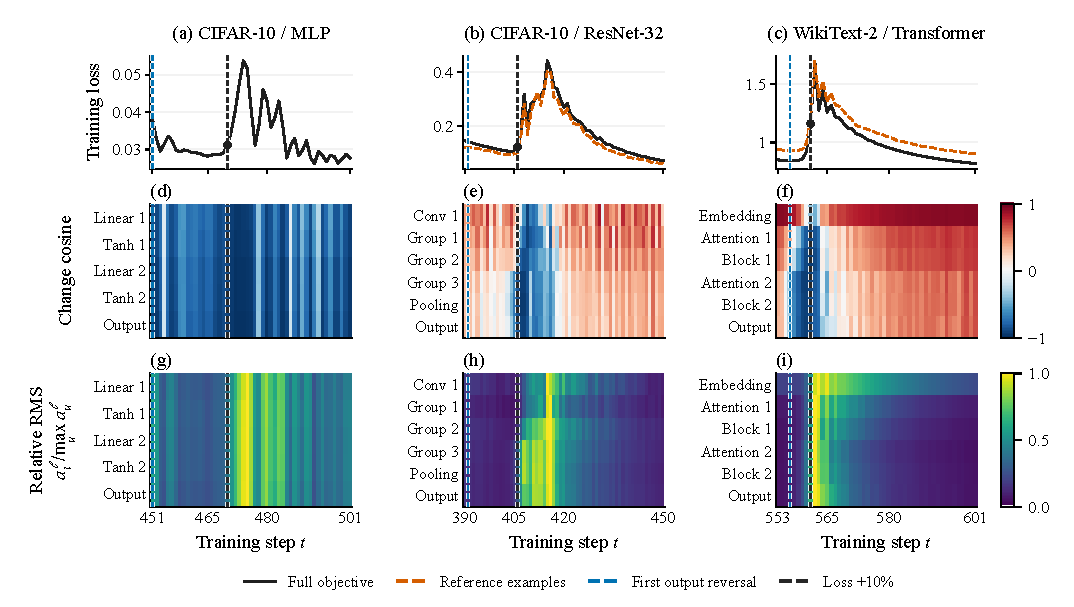
\includegraphics[width=\textwidth]{figures/00-three-model-loss-representation-motion.pdf}
\caption{Loss and representation changes in selected Adam windows: steps 451--501 (MLP), 390--450 (ResNet), and 553--601 (Transformer). Top: complete training loss and loss on the reference examples. Middle: cosine between consecutive representation changes; blue denotes reversal and red denotes reinforcement. Bottom: relative RMS displacement $a_t^\ell/\max_{u\in[a,b]}a_u^\ell$, normalized separately within each site and displayed window. The 5/6/6 rows are measured site outputs, not averages of internal layers. Reference sets contain 5,000 images, one original 1,000-image BatchNorm group, and 2,240 token positions. Blue dashed lines mark the first displayed negative output-change cosine; the MLP is already negative at entry. Black dashed lines mark the first loss at least 10\% above the pre-peak minimum. These lines compare timing; they do not identify a unique initiating event.}
\label{fig:trace-motion}
\end{figure*}

Figure~\ref{fig:trace-motion} shows where functional oscillation appears
and how its size changes. The top row locates the loss excursion.
Reading the cosine maps backwards from output to input reveals how
widely reversal is shared. In the MLP, every displayed change has
negative cosine at every measured site, from the first linear input
map to the final output. Oscillation is therefore homogeneous across
the measured depth, even while loss rises and falls. The RMS maps add
its changing amplitude. Comparing pre- and post-nonlinearity measurements
shows that tanh attenuates displacement; each site's separate
normalization in the figure highlights timing rather than absolute
differences in magnitude across sites.

ResNet and Transformer exhibit a less homogeneous pattern. Their
output-side representations reverse while earlier representations can
continue to reinforce their preceding change. The first displayed output
reversal precedes the 10\% loss marker by 15 steps in ResNet and five
in Transformer. In ResNet, the first convolution reaches its largest
displacement at the loss peak, followed one step later by the remaining
displayed sites. In Transformer, the embedding becomes more oscillatory
near the large excursion and returns to constructive movement sooner
than the later sites. Larger backpropagated errors could recruit earlier
representations into stronger changes, while constructive intervals
could accumulate smaller changes before that reorganization. This
architecture-dependent interpretation motivates examining both the
direction and magnitude throughout the network.

\begin{figure*}[!t]
\centering
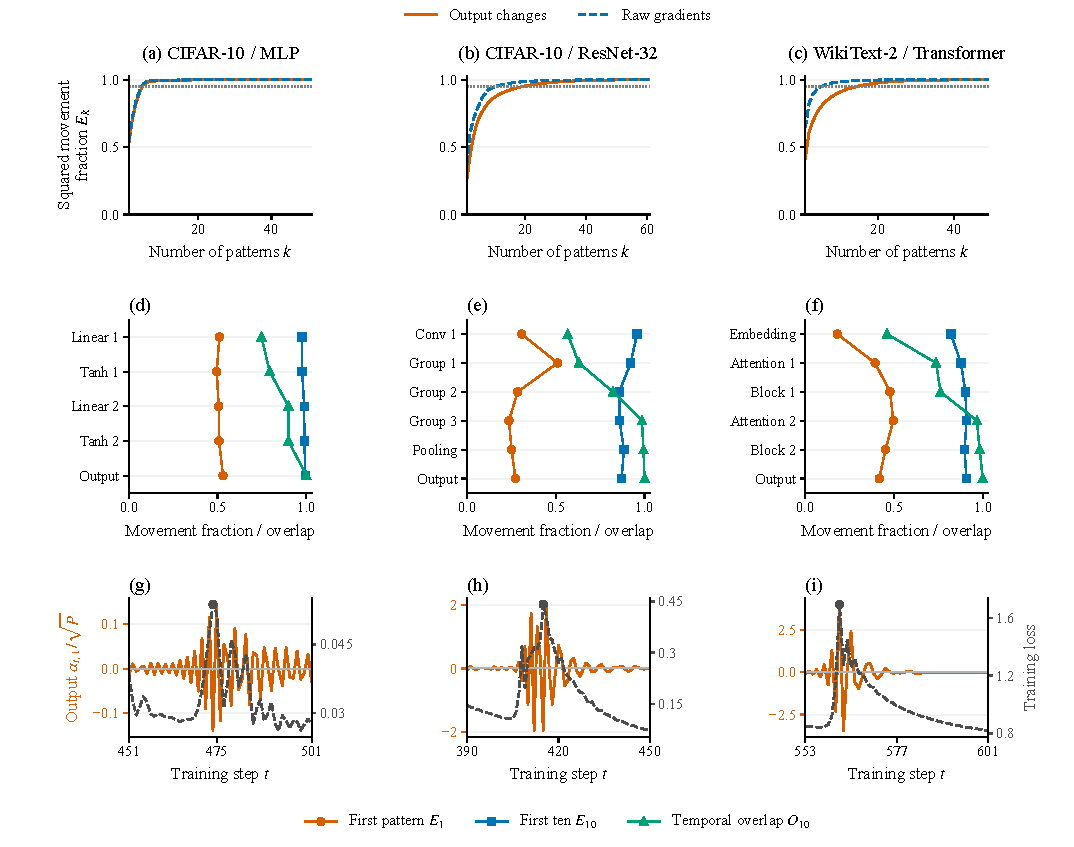
\includegraphics[width=\textwidth]{figures/01-three-model-temporal-structure.pdf}
\caption{Patterns and timing of representation movement in the same windows as Fig.~\ref{fig:trace-motion}, containing 51/61/49 changes. Top: cumulative fraction of squared movement for output changes and for the raw gradients used by those updates; the dotted line marks 95\%. Middle: each site's fraction in its first pattern ($E_1^\ell$) and first ten ($E_{10}^\ell$), and temporal overlap with the output ($O_{10}$). Bottom: signed coefficient of the leading output pattern, divided by $\sqrt P$ to express its coordinate RMS scale. A coefficient crossing zero reverses direction along that fixed pattern. Energy, temporal overlap, and signed motion answer different questions; none alone establishes causal transmission through a layer.}
\label{fig:trace-structure}
\end{figure*}

Figure~\ref{fig:trace-structure} asks whether these changes repeatedly
use a small set of patterns. The top row shows concentration of squared
movement in the leading output modes, alongside the corresponding
gradient decomposition. Concentration can reflect both repeated
directions and a few large changes; the equal-length and orthogonal
controls in Supplementary Section S4 separate these effects.
The middle row extends the analysis through the network: $E_1^\ell$
and $E_{10}^\ell$ show concentration at each site, whereas $O_{10}$ shows
how much its leading temporal structure is shared with the final output.
The selected ResNet window has stronger temporal agreement toward the
output, with shared structure still extending to the input-side sites.
Finally, the bottom row establishes the back-and-forth component that
energy fractions alone cannot establish. Repeated changes in the sign
of $\alpha_{t,1}^F/\sqrt{P_F}$ show reversal along one fixed output
pattern, and its amplitude shows how strongly that pattern moves.

Together, the two figures and the small retention values characterize
coordinated, approximately low-dimensional functional oscillation in
these windows. The temporal Gram matrix $D_\ell D_\ell^\top$ permits
the analysis without storing all spatial modes; implementation and
numerical checks are in Supplementary Section S4. The resulting
intervention question is whether limiting the magnitude of local
representation changes can reduce loss excursions while preserving
subsequent training progress.

% Full-paper adaptation; the separately reviewed V-C fragment remains unchanged.
% Requires amsmath, amssymb, graphicx, booktabs, algorithm, algpseudocode.
\providecommand{\vcassetroot}{../evidence/05-adam/c-intervention}
\subsection{Interventions Guided by Functional Motion}
\label{sec:vc-interventions}

The tracing analysis separates the direction and magnitude of representation
changes. We therefore test whether limiting local displacement can reduce loss
excursions while preserving training progress and allowing reversals. We compare
a local displacement cap with immediate LR reduction, late second-moment
changes, and global gradient clipping.

\begin{figure*}[!t]
\centering
\includegraphics[width=\textwidth]{\vcassetroot/figures/24-main-intervention-tradeoff.pdf}
\caption{Loss variation and training progress for all 33 treated continuations,
each compared with its unchanged Adam control at the origin. Horizontal values
are $100(\bar L/\bar L_{\mathrm{Adam}}-1)$; vertical values are
$100(1-\mathrm{PV}/\mathrm{PV}_{\mathrm{Adam}})$. Leftward and upward changes are
favorable. Axes are model-specific and retain every setting, including increased
variation. This is one initialization per model; settings have unequal effective
strength and are not independent seed replications.}
\label{fig:vc-tradeoff}
\end{figure*}

\input{\vcassetroot/tables/matched-main-outcomes.tex}

\begin{figure*}[!t]
\centering
\includegraphics[width=\textwidth]{\vcassetroot/figures/25-main-q50-functional-motion.pdf}
\caption{Full training loss and fixed-probe motion under unchanged Adam and the
preselected q50 cap. Heatmaps show consecutive-change cosine and displacement
RMS at five MLP and six ResNet/Transformer stage endpoints. Each incoming change
is placed at its completed-step endpoint. Both RMS maps divide by the same
stage-specific maximum under unchanged Adam; the color scale includes every
value. Dashed vertical lines mark the baseline's largest relative loss-excursion
peak within the full window, not treatment triggers. Embed., Attn and Pool denote
embedding, attention output and pooling endpoints. Output motion uses raw MLP
coordinates or cross-entropy log probabilities. No smoothing or stage averaging
is applied.}
\label{fig:vc-motion}
\end{figure*}

\subsubsection{A past-calibrated displacement cap}
For an affine module $Z=HW^\top+\mathbf{1}_n b^\top$, let
$H_s\in\mathbb{R}^{n\times d}$ contain its current fixed-probe inputs,
$W_s\in\mathbb{R}^{m\times d}$ its weights, and $b_s\in\mathbb{R}^m$ its biases.
Rows index examples or token/spatial positions; columns of $Z\in\R^{n\times m}$
index output units. Let $\Delta W_s$ and $\Delta b_s$ be the native stored Adam increments
with the shapes of $W_s$ and $b_s$. Convolution inputs are receptive-field
patches; absent biases have zero increment.
The direct change attributable to this module's update is
\begin{equation}
 \Delta Z_s^{\mathrm{dir}}=H_s\Delta W_s^\top+\mathbf{1}_n \Delta b_s^\top,\qquad
 c_{s,j}=\frac{\|\Delta Z^{\mathrm{dir}}_{s,:,j}\|_2}{\sqrt{n}}.
 \label{eq:vc-score}
\end{equation}
Thus $c_{s,j}$ is one RMS score per output unit across the probe rows,
rather than a worst-case bound for each example. For a positive module budget
$\tau_\ell$, we scale each complete output-unit
weight row and its bias together:
\begin{equation}
 \begin{split}
 a_{s,j}&=\min(1,\tau_\ell/c_{s,j}),\\
 \Delta W^{\mathrm{cap}}_{s,j:}&=a_{s,j}\Delta W_{s,j:},\qquad
 \Delta b^{\mathrm{cap}}_{s,j}=a_{s,j}\Delta b_{s,j}.
 \end{split}
 \label{eq:vc-cap}
\end{equation}
A zero score uses factor one; a zero budget disables that module's cap.
Before treatment at step $f\to f+1$, one scalar budget per module is fixed as
\begin{equation}
 \begin{split}
 \tau_\ell(q)&=\operatorname{Quantile}_q\{c^{\mathrm{native},\ell}_{s,j}\},\\
 &s=f-8,\ldots,f-1,\quad j=1,\ldots,m_\ell.
 \end{split}
 \label{eq:vc-calibration}
\end{equation}
Quantiles use linear interpolation of the pooled scores. The median (q50)
is preselected; q25/q75 test sensitivity. Units whose proposal would induce
larger direct movement are damped proportionally, while smaller proposals
are retained. The budget has activation units and remains fixed as the current
inputs change.

The rule bounds direct affine RMS on the current probe, up to FP32 storage
rounding. Incoming upstream motion and its interaction with the update remain
unconstrained, so total representation motion and loss are not bounded.
Algorithm~\ref{alg:vc-cap} retains native Adam state and untargeted increments.
Scores use a current probe forward to capture $H_s$ and local products with
the proposed increments; each module does not require a second full-network
forward at altered weights. Evaluating propagated motion separately compares
successive probe captures. The controller requires neither temporal SVD nor
a matrix inverse, but its extra forward, products, and bookkeeping have measured
cost. Supplementary Section S5 gives the input-metric interpretation and the
unconstrained upstream terms.

\begin{algorithm}[!b]
\caption{Past-calibrated local displacement cap}
\label{alg:vc-cap}
\begin{algorithmic}[1]
\Require State $\theta_s$, Adam state, fixed probe, targets, fixed budgets $\tau_\ell$
\State Compute the full objective gradient at $\theta_s$.
\State Capture current probe inputs $H_s^\ell$ with the fixed normalization context; preserve random state.
\State Advance native Adam moments/clock and retain the actual stored proposal increments.
\For{each target $\ell$ with $\tau_\ell>0$}
  \State Compute scores by~\eqref{eq:vc-score}; scale weight rows and biases by~\eqref{eq:vc-cap}.
\EndFor
\State Store $\theta_{s+1}$ with untargeted increments unchanged; retain the advanced Adam state.
\State Check direct-score bounds with storage-rounding tolerance; measure propagated motion and loss separately.
\end{algorithmic}
\end{algorithm}

\subsubsection{Matched comparison}
Within each model, all settings share complete model/optimizer/random state,
data order and numerical settings at one initialization. Fixed windows are
$512$--$800$ for CIFAR-10/MLP,
$256$--$576$ for CIFAR-10/ResNet-32, and $544$--$928$ for the two-layer
WikiText-2 Transformer. Training step $s$ counts completed optimizer updates.
Each update uses the complete objective in Table~\ref{tab:setup}, with its
original normalization groups and no dropout.

Unchanged Adam~\cite{kingma2014adam} uses learning rates $.001/.003/.003$,
$\beta_1=.9$, $\beta_2=.999$, $\epsilon=10^{-8}$, and no weight decay.
The four intervention families are immediate LR multipliers $.75/.5/.1$;
late $\beta_2$ values $.95/.9/.5$; global raw-gradient L2 clipping at
$.5/1$~\cite{pascanu2013difficulty}; and distributed q25/q50/q75 caps.
The $\beta_2$ switch retains moments and the step counter, using the new value
in both the recurrence and native $1-\beta_2^{\mathrm{step}}$ correction.
Clipping acts on the complete accumulated raw gradient before Adam.
Caps target both MLP hidden affines, all 31 ResNet convolutions, and the two
QKV and four feed-forward Transformer affines. All 12 conditions per model
start at the same fork; no intervention waits for a later detected spike.

Probes retain the coverage in Table~\ref{tab:setup}.
The full training gradient is unchanged by probe coverage. Every state has loss
and motion measurements. FP32 training/storage and FP64 reductions are matched;
exact native replay checks qualify shared controls across workers.

We report the mean post-fork loss $\bar L$ and positive loss variation,
\begin{equation}
 \bar L=\frac{1}{e-f}\sum_{s=f+1}^{e}L_s,\qquad
 \mathrm{PV}=\sum_{s=f+1}^{e}\max(L_s-L_{s-1},0).
 \label{eq:vc-outcomes}
\end{equation}
PV accumulates upward loss changes, rather than counting excursions.
Final training loss, the last-32-state mean and full held-out losses retain
endpoint context. Held-out evaluations at $f$, $f+32$, midpoint, $e-32$ and $e$
are not used to select checkpoints or settings.

\subsubsection{Excursion suppression and training progress}
Figure~\ref{fig:vc-tradeoff} and Table~\ref{tab:vc-outcomes} separate loss
smoothness from learning progress. Reducing LR to $.1\eta$ removes
$99.6\%$, $99.0\%$, and $100\%$ of PV in MLP/ResNet/Transformer, but increases
ResNet mean loss by $89.5\%$. Late $\beta_2$ changes are model-dependent:
all three worsen MLP mean loss and PV, whereas $\beta_2=.9$ lowers
Transformer mean loss by $16.8\%$. Both clipping thresholds worsen mean loss
and PV in MLP and ResNet. Transformer clipping at $.5$ instead lowers them
by $17.8\%$ and $87.7\%$, respectively.

All nine cap/model combinations lower both mean loss and PV. The lowest observed
mean loss in each model belongs to a cap setting: q50 for MLP/Transformer
and q25 for ResNet. The preselected q50 reduces mean loss by
$32.2\%$, $9.4\%$, and $19.8\%$, with PV reductions of $87.8\%$, $2.8\%$, and $96.2\%$.
Quantile sensitivity is nonmonotone, and the finite-window mean does not establish
better terminal convergence. In particular, ResNet q50 increases final and
last-32 loss by $20.0\%$ and $21.5\%$; q25/q75 improve those endpoints.
The full trajectories and detailed outcomes are retained in the supplementary
comparison.

\subsubsection{Functional effect and limits}
Figure~\ref{fig:vc-motion} shows that q50 lowers the largest output RMS jump
by $83.2\%$, $23.1\%$, and $62.9\%$, while output reversals remain at
$89.2\%$, $66.9\%$, and $95.8\%$ of updates. Their baseline frequencies are
$99.3\%$, $36.9\%$, and $36.7\%$. Smaller extreme jumps therefore coexist with
persistent, sometimes more frequent, reversals. Total squared output motion
falls $88.6\%$ and $55.4\%$ in MLP and Transformer, but rises $39.7\%$
in ResNet. The effect concerns extreme displacements, not uniform suppression
of every measure of motion.

In the previously selected ResNet tracing window, steps $390$--$450$, q50
reduces the maximum loss from $.4407$ to $.1736$ ($60.6\%$).
Later oscillations explain why the complete $256$--$576$ window has only
$2.8\%$ lower PV. This secondary readout connects the intervention to the
traced event while retaining the full horizon as the primary comparison.

\begin{samepage}
For the squared-loss MLP, actual output motion has the exact accounting
\begin{equation}
 L_{s+1}-L_s=\frac{\langle F_s-Y,\Delta F_s\rangle}{N}
             +\frac{\|\Delta F_s\|_F^2}{2N},
 \label{eq:vc-output-loss}
\end{equation}
\end{samepage}
where $\Delta F_s=F_{s+1}-F_s$ and $N=5000$. For all 161 baseline and
70 q50 output-space loss rises above $10^{-8}$, the linear term is negative
and outweighed by the quadratic term. This is an exact output-space identity;
its linear term need not equal the parameter-space directional derivative.
Cross-entropy requires its own readout. The evidence supports displacement
control with persistent reversals, without identifying a unique causal source.

Training improvements also carry held-out tradeoffs: q50 terminal test loss
increases $0.53\%$, $2.42\%$, and $27.52\%$. These evaluations cover all 10,000
CIFAR-10 test images and 245,550 WikiText-2 test tokens; full validation and
five-state trajectories accompany the supplementary results. The implementation
has measurable cost: in the MLP q50 arm, controller time is $41.8$ ms/update,
compared with $4.4$ ms/full-gradient boundary. Instrumentation and host differences
preclude a time-to-loss claim. These single-initialization continuations use
unequal effective intervention strengths; reliability across initializations,
stochastic deployment and generalization benefits require additional evidence.

